\documentclass{article}

\usepackage{bbm}
\usepackage{fancyhdr}
\usepackage{titling}
\usepackage{enumitem}
\usepackage{amsmath}
\usepackage{dsfont}
\usepackage{amsfonts}
\usepackage{amssymb}
\usepackage{amsthm}
\usepackage{geometry}
\usepackage{tikz}
\usepackage{algorithm}
\usepackage{algpseudocode}
\geometry{verbose,tmargin=1in,bmargin=1in,lmargin=1in,rmargin=1in}
\renewcommand{\vec}[1]{\mathbf{#1}}
\newcommand{\dec}{\text{dec}}
\newcommand{\divi}{\mathbin{\textnormal{div}}}
\title{Homework 1}
\author{Satvik Prasad}
\date{}
\newtheorem{lemma}{Lemma}[section]
\fancypagestyle{plain}{%
  \fancyhf{}
  \fancyhead[L]{\theauthor}
  \fancyhead[R]{\thedate}
}
\pagestyle{plain}
\makeatletter
\def\@maketitle{%
  \newpage
  \null
  \vskip 1em%
  \begin{center}%
    \let \footnote \thanks
    {\LARGE \@title \par}%
    \vskip 1em%
  \end{center}%
  \par
\vskip 1em}
\makeatother
\usepackage{cmbright}

\newcommand{\mat}[1]{\mathbf{#1}}

% ---------- Probability theory ----------
% Core operators (optional argument-free; use as \E{X}, \Var{X}, \Cov{X}{Y})
\DeclareMathOperator{\EOp}{\mathbb{E}}
\DeclareMathOperator{\VarOp}{Var}
\DeclareMathOperator{\CovOp}{Cov}
\DeclareMathOperator{\CorrOp}{Corr}

\renewcommand{\P}[1]{\mathbb{P}\left(#1\right)}        % \P{A}
\newcommand{\E}[1]{\EOp\left[#1\right]}                % \E{X}
\newcommand{\Var}[1]{\VarOp\left(#1\right)}            % \Var{X}
\newcommand{\Cov}[2]{\CovOp\left(#1,\,#2\right)}       % \Cov{X}{Y}
\newcommand{\Corr}[2]{\CorrOp\left(#1,\,#2\right)}     % \Corr{X}{Y}
\newcommand{\SD}[1]{\operatorname{SD}\left(#1\right)}  % \SD{X}

% Subscripted versions, e.g. \Esub{\theta}{X}, \Psub{\theta}{A}
\newcommand{\Esub}[2]{\EOp_{#1}\left[#2\right]}
\newcommand{\Psub}[2]{\mathbb{P}_{#1}\left(#2\right)}

% Conditioning, indicators, independence
\newcommand{\given}{\,\middle|\,}                      % \E{X \given Y}
\newcommand{\ind}[1]{\mathbbm{1}\left\{#1\right\}}     % \ind{X > 0}
\newcommand{\indep}{\perp\!\!\!\perp}                  % X \indep Y
\newcommand{\iid}{\overset{\text{iid}}{\sim}}          % X_i \iid \Normal(0,1)

% Convergence
\newcommand{\convp}{\xrightarrow{\;p\;}}               % in probability
\newcommand{\convd}{\xrightarrow{\;d\;}}               % in distribution
\newcommand{\convas}{\xrightarrow{\text{a.s.}}}        % almost surely
\newcommand{\convLp}[1]{\xrightarrow{L^{#1}}}          % in L^p

% Probability spaces
\newcommand{\F}{\mathcal{F}}                           % sigma-algebra
\newcommand{\B}{\mathcal{B}}                           % Borel sigma-algebra
\newcommand{\pspace}{(\Omega, \F, \mathbb{P})}

% Common distributions
\newcommand{\Normal}{\mathcal{N}}
\newcommand{\Bern}{\operatorname{Bernoulli}}
\newcommand{\Bin}{\operatorname{Binomial}}
\newcommand{\Pois}{\operatorname{Poisson}}
\newcommand{\Unif}{\operatorname{Uniform}}
\newcommand{\Exp}{\operatorname{Exp}}
\newcommand{\Geom}{\operatorname{Geometric}}
\newcommand{\Gam}{\operatorname{Gamma}}
\newcommand{\Beta}{\operatorname{Beta}}

% Number sets
\newcommand{\R}{\mathbb{R}}
\newcommand{\N}{\mathbb{N}}
\newcommand{\Z}{\mathbb{Z}}


 \title{Homework 10}
\author{Math 3012}
\date{Updated 2026}

\begin{document}

\begin{enumerate} 
\item We use Prim's algorithm on the original graph, starting at vertex $f.$ This process yields the following minimum spanning tree:
    \begin{center}
    \begin{tikzpicture}[scale=1]
        \tikzstyle{vertex}=[circle, fill=black, inner sep=1.5pt]
        \tikzstyle{weight}=[text=blue, midway]
    
        % Define nodes in a hexagon
        \node[vertex] (a) at (0, 0) [label=below:$a$] {};
        \node[vertex] (b) at (4, 0) [label=below:$b$] {};
        \node[vertex] (c) at (6, 3.46) [label=right:$c$] {};
        \node[vertex] (d) at (4, 6.92) [label=above:$d$] {};
        \node[vertex] (e) at (0, 6.92) [label=above:$e$] {};
        \node[vertex] (f) at (-2, 3.46) [label=left:$f$] {};
    
        % Outer edges
        \draw (a) -- (b) node[weight, below] {3};
        \draw (b) -- (c) node[weight, below right] {1};
        \draw (c) -- (d) node[weight, above right] {1};
        \draw (d) -- (e) node[weight, above] {2};
        \draw (e) -- (f) node[weight, above left] {1};
    
        % Inner edges
    \end{tikzpicture}
    \end{center}
 
\item We start with the following graphs, and attempt to determine whether the graphs are isomorphic or not.

\begin{figure}[htb]
    \centering
    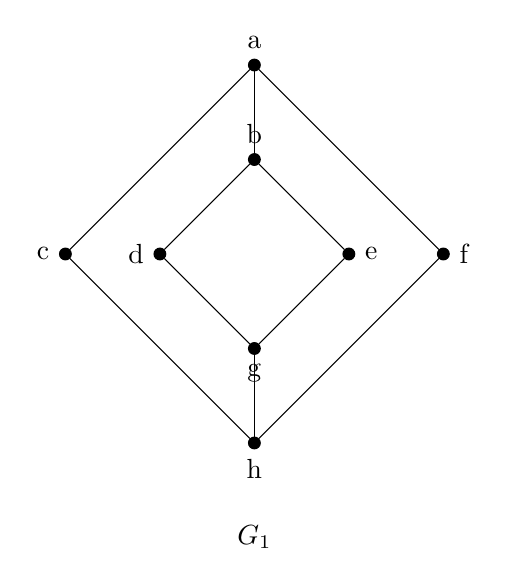
\begin{tikzpicture}[scale=0.8]
        % Graph 1 (Left)
        \node[draw, circle, fill=black, inner sep=1.5pt] (a) at (0, 3) [label=above:a] {};
        \node[draw, circle, fill=black, inner sep=1.5pt] (h) at (0, -3) [label=below:h] {};
        \node[draw, circle, fill=black, inner sep=1.5pt] (c) at (-3, 0) [label=left:c] {};
        \node[draw, circle, fill=black, inner sep=1.5pt] (f) at (3, 0) [label=right:f] {};
        \node[draw, circle, fill=black, inner sep=1.5pt] (b) at (0, 1.5) [label=above:b] {};
        \node[draw, circle, fill=black, inner sep=1.5pt] (g) at (0, -1.5) [label=below:g] {};
        \node[draw, circle, fill=black, inner sep=1.5pt] (d) at (-1.5, 0) [label=left:d] {};
        \node[draw, circle, fill=black, inner sep=1.5pt] (e) at (1.5, 0) [label=right:e] {};

        \node (X) at (0, -4) [label=below:$G_1$] {};
        
        % Edges for G1
        \draw (a) -- (c) -- (h) -- (f) -- (a);
        \draw (b) -- (d) -- (g) -- (e) -- (b);
        \draw (a) -- (b);
       
        \draw (h) -- (g);
         
    \end{tikzpicture}
    \qquad\qquad % Space between graphs
    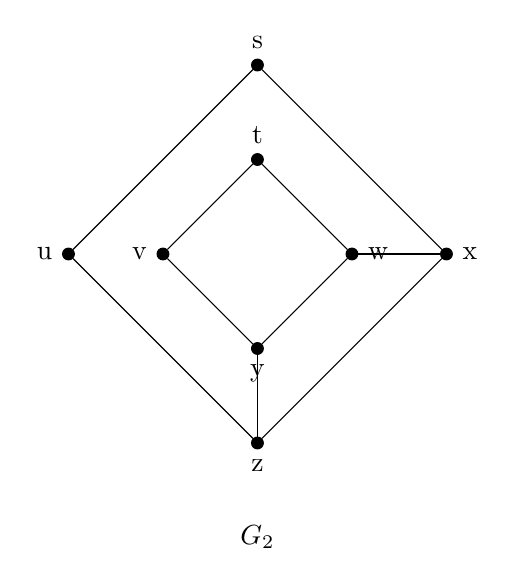
\begin{tikzpicture}[scale=0.8]
        % Graph 2 (Right)
        \node[draw, circle, fill=black, inner sep=1.5pt] (s) at (0, 3) [label=above:s] {};
        \node[draw, circle, fill=black, inner sep=1.5pt] (z) at (0, -3) [label=below:z] {};
        \node[draw, circle, fill=black, inner sep=1.5pt] (u) at (-3, 0) [label=left:u] {};
        \node[draw, circle, fill=black, inner sep=1.5pt] (x) at (3, 0) [label=right:x] {};
        \node[draw, circle, fill=black, inner sep=1.5pt] (t) at (0, 1.5) [label=above:t] {};
        \node[draw, circle, fill=black, inner sep=1.5pt] (y) at (0, -1.5) [label=below:y] {};
        \node[draw, circle, fill=black, inner sep=1.5pt] (v) at (-1.5, 0) [label=left:v] {};
        \node[draw, circle, fill=black, inner sep=1.5pt] (w) at (1.5, 0) [label=right:w] {};

        \node (X) at (0, -4) [label=below:$G_2$] {};
        
        % Edges for G2
        \draw (s) -- (u) -- (z) -- (x) -- (s);
        \draw (t) -- (v) -- (y) -- (w);
        
         
        \draw (z) -- (y);
        \draw (x) -- (w);
        \draw (t) -- (w);
    \end{tikzpicture}
\end{figure}
Now, we notice that the number of subgraphs of $G_1$ that are isomorphic to $C_4$ is 2, namely the graphs $$(\{b, e, d, g\}, \{[b, e], [e, g], [g, d], [d, b]\}), \qquad (\{a, f, h, c\}, \{[a, f], [f, h], [h, c], [c, a]\}).$$ However, the number of subgraphs of $G_2$ that are isomorphic to $C_4$ is 3, namely \begin{align*}
    (\{x, w, y, z\}, \{[x, w], [w, y], [y, z], [z,x]\}), \qquad (\{w, t, v, y\}, \{[w, t], [t, v], [v, y], [y, w]\}),
\end{align*}
and $$(\{s, x, z, u\}, \{[s, x], [x, z], [z, u], [u, s]\}).$$
Since for all graphs $F,$ isomorphic graphs must have the same number of subgraphs isomorphic to $F,$ we can conclude that $G_1$ and $G_2$ are not isomorphic.

\newpage
\item An Eulerian trail does exist, since there are 2 vertices with odd degree $(a, b)$ and the rest have even degree. 

\begin{center}
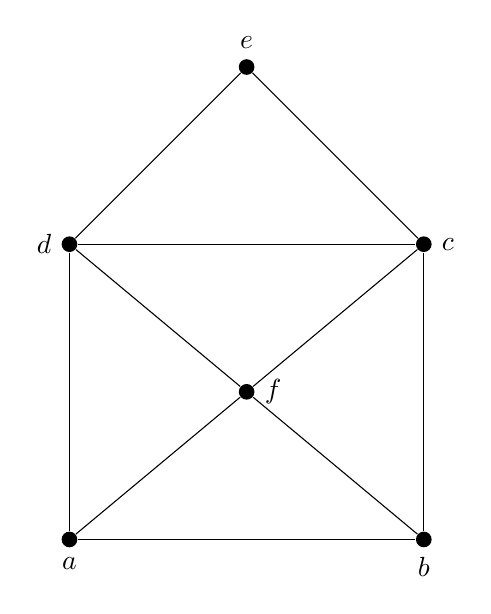
\begin{tikzpicture}[scale=1.5, auto, swap]
    \tikzstyle{vertex}=[circle, fill=black, inner sep=2pt]
    \node[vertex] (a) at (0,0) [label=below:$a$] {};
    \node[vertex] (b) at (3,0) [label=below:$b$] {};
    \node[vertex] (c) at (3,2.5) [label=right:$c$] {};
    \node[vertex] (d) at (0,2.5) [label=left:$d$] {};
    \node[vertex] (e) at (1.5,4) [label=above:$e$] {};
    \node[vertex] (f) at (1.5,1.25) [label=right:$f$] {};

    \draw (a) -- (b); \draw (b) -- (f); \draw (f) -- (a);
    \draw (a) -- (d); \draw (b) -- (c); \draw (c) -- (d);
    \draw (d) -- (e); \draw (e) -- (c); \draw (c) -- (f); \draw (d) -- (f);
\end{tikzpicture}
\end{center}
Our Eulerian trail must begin at one of $(a, b),$ and end at the other. Listing the vertices and omitting the edges for our trail (since for any pair $(u, v)$ there is at most one unique from $u$ to $v$), we can take the edges in order $$b, c, e, d, f, c, d, a, f, b, a.$$


\item  We want to count the number of paths $P_n$  in the complete graph $K_n.$ We first prove that there is a bijection from the number of paths $P_n$ in the complete graph $K_n,$ to the permutations of the numbers $1,2, \ldots n,$ where the first element of the permutation is less than the last.

Notice that each permutation $p = (p_1, p_2, \ldots, p_n),$ $p_1 < p_n,$ of the numbers $1, \ldots, n$ can be mapped to a unique path $$P = (\{1, \ldots, n\}, \{[p_1, p_2], [p_2, p_3], \ldots, [p_{k-1}, p_k]\}).$$ In other words, we construct a mapping $f: \{s \in S_n \mid s_1 < s_n\} \rightarrow \{P \mid P \in P_n, P \subseteq K_n\}$ given by \begin{align*}
    \qquad f(p_1, \ldots, p_n) = (\{1, \ldots, n\}, \{[p_1, p_2], [p_2, p_3], \ldots [p_{k-1}, p_k]\}).
\end{align*}
We know $f(p_1, \ldots p_n)$ is a subgraph of $K_n$ since edges in the form $[p_r, p_{r + 1}]$ are guaranteed to exist, since $K_n$ is complete. Additionally, it is a path since $2$ vertices $p_1 p_k$ have degree $1,$ and the rest have degree $2.$

Now, we show that $f$ is bijective. We know this map is injective since two distinct permutations are guaranteed to produce two distinct paths, since their edge sets will be distinct. Secondly, this map is surjective since every path can be written with its edges in successive order, starting from the node with degree $1$ with the least label, and then listing in order, i.e in the form $$P = (\{1, \ldots, n\}, \{[p_1, p_2], [p_2, p_3], \ldots [p_{k-1}, p_k]\}), \qquad p_1 < p_k.$$
Then, with $P$ in this form we know the permutation $\mathcal P = (p_1, \ldots p_k)$ satisfies $p_1 < p_k$ and thus maps to $P,$ i.e $f(\mathcal P) = P.$ Thus, since $f$ is both injective and surjective, it is bijective.

Therefore, to count the number of paths $P_n$ in the complete graph $K_n,$ we just need to count the number of permutations where the leading element is less than the trailing element. To count this quantity, we first pick the first and last elements in $n \choose 2$ ways. Once chosen, their relative order is locked since the larger element cannot be the first. Then, we permute the remaining $n-2$ elements between themselves, in $(n-2)!$ ways. Hence, the cardinality of this set is equal to \begin{align*}
{n \choose 2} \cdot  (n-2)! = \dfrac{n(n-1)}{2} \cdot (n-2)! = \dfrac{n!}{2}.
\end{align*}
Thus, the number of unique paths $P_n$ in the complete graph $K_n$ is $n!/2.$
\end{enumerate}
\end{document}